\section{Recurent Neural Network}

\gls{RNN}
Réseau de neurones avec une boucle temporelle.
La couche cachée produit une sortie à la fois vers le dernier niveau mais renvoit également sa sortie dans son entrée.

\begin{figure}[ht]
	\centering
	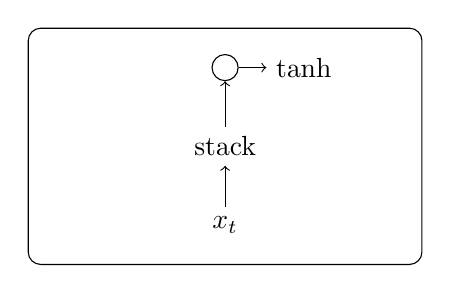
\begin{tikzpicture}
		\draw[rounded corners=4.5pt] (0, 0) rectangle (5, 3);

		\node[circle, draw] (node) at (2.5, 2.5) {};
		\node (stackfunc) at (2.5, 1.5) {stack};
		\node (outputfunc) at (3.5, 2.5) {tanh};
		\node (entry) at (2.5, .5) {$x_t$};

		\draw[->] (node) -- (outputfunc);
		\draw[->] (stackfunc) -- (node);
		\draw[->] (entry) -- (stackfunc);
	\end{tikzpicture}
	\caption{Représentation simplifiée d'un réseau de neurones récurrent}
\end{figure}

\paragraph{One to Many}

\paragraph{Many to One}

\subsection{\gls{LSTM}}

\paragraph{forget gate}
\begin{equation}
	f_t = \sigma(W_f [h_{t-1}, x_t] + b_f)
\end{equation}